\chapter{Resultados predictivos: qué aprendió el sistema}
\label{chap:resultados}

Los dos capítulos anteriores describieron un mecanismo y un protocolo. Éste responde a la primera de
las dos preguntas empíricas del trabajo: ¿existe realmente la ordenación que el sistema dice haber
aprendido, y resiste los contrastes que tratan de explicarla por azar?

El capítulo se ocupa exclusivamente de evidencia \emph{predictiva}. Toda cifra económica que aparece
aquí --- y aparecen algunas, porque ciertos contrastes de robustez se construyen sobre carteras ---
tiene carácter diagnóstico y no debe confundirse con la evaluación económica del
Capítulo~\ref{chap:resultados-economicos}, que se hace con una cartera distinta y elegida por otro
criterio. Cada tabla declara su procedencia.

El orden es deliberado: primero qué configuración eligió el protocolo, después qué aprendió el
meta-agente y cada especialista, luego la capacidad predictiva agregada y su comparación con
baselines, y por último los contrastes adversariales.
\section{La configuración ganadora y la cadena de estudios}
\label{sec:configuracion-ganadora}

La evidencia de este capítulo procede del tercer Model Study de la cadena, y conviene fijar antes de
nada de dónde sale cada cifra. El protocolo del capítulo anterior no se aplicó una vez sino tres,
encadenadas: el ganador de cada pasada se convierte en el punto de partida de la siguiente. Los tres
estudios comparten ventana de selección, era reservada y métrica, y se diferencian únicamente en ese
punto de partida.

\begin{table}[H]
  \centering
  \small
  \caption{Las tres pasadas de la cadena y su ganador.}
  \label{tab:cadena}
  \begin{tabular}{llrrrrrrr}
\toprule
Pasada & Run ganador & Rank-IC & IC-IR & $t$ NW & Transf. & IR sel. & Exceso sel. & IR reserv. \\
\midrule
Study 1 & run-6eaa47a0597b & 0,1000 & 0,735 & 2,95 & 0,178 & 0,189 & 1,07\% & 0,898 \\
Study 2 & run-2dc586be8653 & 0,1074 & 0,835 & 3,36 & 0,234 & 0,294 & 1,89\% & 0,476 \\
Study 3 & run-f134d7eb9e06 & 0,1090 & 0,851 & 3,46 & 0,328 & 0,339 & 2,61\% & -1,167 \\
\bottomrule
\end{tabular}

  \caption*{Fuente: \artefacto{winner.json}, \artefacto{evidence/summary.json} y
  \artefacto{attribution.json} de cada pasada. Rank-IC, IC-IR y $t$ de Newey--West son de la ventana
  de selección; IR y exceso corresponden a la cartera \emph{por defecto} de cada estudio, no a la
  optimizada del Capítulo~\ref{chap:resultados-economicos}.}
\end{table}

Dos lecturas de esta tabla condicionan todo el capítulo. La primera es que la cadena mejoró de forma
monótona dentro de la ventana de selección: el Rank-IC pasa de 0,1000 a 0,1074 y a 0,1090, y la
transferencia de 0,178 a 0,328. La segunda es que la última columna va en dirección contraria ---
0,898, 0,476 y $-1{,}167$ de Information Ratio fuera de la ventana de decisión ---, un patrón que
tiene la forma exacta del sobreajuste por búsqueda y que el Capítulo~\ref{chap:resultados-economicos}
examina en detalle, porque su explicación resultó no estar en el modelo.

\begin{table}[H]
  \centering
  \small
  \caption{Qué cambió cada pasada respecto de su punto de partida.}
  \label{tab:cadena-config}
  \begin{tabular}{lrp{0.62\linewidth}}
\toprule
Pasada & Cambios & Variables modificadas respecto del punto de partida \\
\midrule
Study 1 & 9 & commission\_bps, coverage\_percentile\_floor, feature\_preset, max\_features\_per\_agent, meta\_method, minimum\_holding\_period, slippage\_bps, snapshot\_step\_months, target\_size \\
Study 2 & 2 & lgbm\_min\_child\_samples, max\_features\_per\_agent \\
Study 3 & 2 & lgbm\_learning\_rate, market\_regime\_feature \\
\bottomrule
\end{tabular}

  \caption*{Fuente: \artefacto{winner.json} de cada pasada, comparado con la configuración de
  partida. El Anexo~\ref{anexo:catalogo} reproduce el catálogo completo con el valor final de las
  treinta y tres variables.}
\end{table}

La Tabla~\ref{tab:cadena-config} muestra en qué sentido la cadena convergió: la primera pasada se
apartó en ocho variables del baseline recomendado del catálogo, la segunda cambió una sola y la
tercera dos, de las cuales sólo una es predictiva. Esa desaceleración es la que justifica detenerse
en tres pasadas, y es también la razón de que la traza de decisiones del capítulo anterior sea casi
plana.

La configuración ganadora resultante emplea cadencia mensual de snapshots, horizonte de etiqueta de
doce meses, el preset de variables \texttt{all} con un máximo de veinte por agente, sin neutralización
sectorial ni ponderación por recencia, y un meta-agente \texttt{stacked\_rolling\_free}, es decir,
sin tope por agente. Esa última elección procede de la segunda pasada y gobierna buena parte de lo
que sigue; la tercera volvió a compararla con la variante acotada y la confirmó. La
Sección~\ref{sec:cadena-studies} documenta por qué se encadenaron los estudios y qué se aprendió en
cada uno.

\section{La evidencia de que el meta aprende}
\label{sec:meta-aprende}

El aprendizaje es observable, no una afirmación inferida de la rentabilidad final. Las primeras
filas de \texttt{meta\_weights.parquet} corresponden a \texttt{fallback\_equal}: cada agente recibe
0,20 porque aún no existe evidencia cerrada. Después aparecen las filas \texttt{learned}, y en ellas
el peso de \textit{risk} crece de forma sostenida a medida que se cierran cohortes: 0,22 de media en
2016, 0,45 en 2017, 0,66 en 2018, 0,83 en 2020 y valores en torno a 0,95 desde 2022. Al final de la
serie el reparto es prácticamente degenerado --- 0,954 para \textit{risk} y 0,047 para
\textit{value}, con los tres agentes restantes en cero ---, de modo que el meta-agente no aprendió a
combinar cinco especialistas sino a descartar cuatro.

Ese desenlace merece leerse con cuidado, porque es el resultado esperable del método y no una
anomalía. La configuración ganadora emplea \texttt{stacked\_rolling\_free}, es decir, un apilado sin
tope por agente; enfrentado a un especialista que domina de forma consistente, el procedimiento
converge a él. La primera pasada de la cadena usaba la variante acotada; la segunda adoptó la libre
y la tercera volvió a medir ambas y la ratificó, con $+0{,}00827$ de ventaja pareada sobre la
acotada. Se ganó Rank-IC, por tanto, a costa de que la arquitectura multi-agente quede en la
práctica reducida a uno.

El contraste relevante conserva exactamente los mismos cinco agentes y cambia sólo la regla de
combinación. En la ventana de selección, el meta aprendido alcanza Rank-IC 0,1090 frente a 0,0675
del promedio equiponderado: una mejora de 0,0415, equivalente al 61\,\%. La capa de combinación
añade, por tanto, información útil y no sólo reescala los scores.

\begin{table}[H]
  \centering
  \caption{Capacidad predictiva de los agentes y combinadores en 2015--2024.}
  \label{tab:agentes}
  \begin{tabular}{lrrrr}
\toprule
Señal & Rank-IC & Desv. & Positivas & IC-IR \\
\midrule
risk & 0,1227 & 0,1241 & 80,34\% & 0,988 \\
meta\_final & 0,1090 & 0,1281 & 74,36\% & 0,851 \\
meta\_equal\_weight & 0,0675 & 0,1261 & 62,39\% & 0,535 \\
growth & 0,0249 & 0,0865 & 61,54\% & 0,289 \\
value & 0,0244 & 0,0803 & 63,25\% & 0,303 \\
quality & 0,0096 & 0,1051 & 47,01\% & 0,091 \\
momentum & 0,0005 & 0,0902 & 47,86\% & 0,006 \\
\bottomrule
\end{tabular}

  \caption*{Fuente: \artefacto{evidence/rank\_ic\_diagnostics.parquet}. Desviación e IC-IR se
  calculan sobre cohortes cerradas de la ventana de selección.}
\end{table}

Hay, sin embargo, un resultado que este trabajo debe reportar aunque incomode a su propia
arquitectura: \textbf{el agente \textit{risk} por separado ordena mejor que el meta-agente}. Su
Rank-IC es 0,1227 con IC-IR 0,988 y 80,34\,\% de cohortes positivas, frente a 0,1090, 0,851 y
74,36\,\% del meta. La diferencia es pequeña, pero va en la dirección contraria a la que
justificaría la complejidad añadida, y no puede atribuirse al tope de los pesos: con la variante
libre el meta puede concentrarse cuanto quiera y aun así ordena algo peor.

La explicación está en el trayecto. El meta converge hacia \textit{risk} pero tarda años en hacerlo,
y durante ese tiempo arrastra el peso de agentes que ordenan mucho peor --- \textit{quality} 0,0096
y \textit{momentum} 0,0005, ambos indistinguibles de cero ---. Ese coste es irrecuperable porque
forma parte de lo que significa aprender sin mirar al futuro: la superioridad de \textit{risk} se
conoce \emph{a posteriori}, mirando la ventana completa, mientras que el meta la descubrió
progresivamente y sin información futura. Elegir \textit{risk} de antemano no era una opción
disponible en 2015.

La lectura honesta, entonces, tiene dos mitades que deben ir juntas. El meta-agente demuestra saber
\emph{aprender} de la evidencia --- supera con holgura a la combinación ingenua y reproduce casi
toda la señal del especialista dominante sin conocerlo de antemano ---, pero estos datos no
demuestran que combinar aporte más que seleccionar bien. El documento no presenta, por tanto, la
arquitectura multi-agente como demostrada.

\subsection*{Qué significa que el meta se concentre casi por completo}

Que el peso de \textit{risk} termine rozando la unidad es un resultado ambivalente. Leído a favor,
el aprendizaje funciona: el sistema identifica a su mejor especialista en unos dos años, partiendo
de la ignorancia, y mantiene esa identificación de forma estable en lugar de oscilar entre
candidatos. Leído en contra, la arquitectura multi-agente se vacía de contenido en su propio
ganador. Un meta que asigna el 95\,\% del peso a un único agente ha dejado de ser un combinador para
ser un selector.

La variante acotada existía precisamente para evitar este desenlace, y adoptar la libre es un caso
claro de decisión que mejora la métrica de selección a costa de una propiedad cualitativa del
diseño que ninguna métrica del protocolo estaba midiendo. El riesgo que la restricción cubría sigue
existiendo y queda asumido: la señal del sistema es, en la práctica, la del agente \textit{risk}, de
modo que su comportamiento futuro depende de que ese especialista siga funcionando. La era reservada
permite una primera comprobación --- el Rank-IC se mantiene positivo en $+0{,}0441$ ---, pero seis
cohortes no bastan para descartar que la concentración sea frágil. Queda recogido como limitación en
el Capítulo~\ref{chap:limitaciones}.

Una advertencia de lectura afecta a todo el capítulo. Los artefactos contienen dos ventanas para
esta misma métrica: la de \emph{selección}, con 117 cohortes hasta 2024, y la \emph{completa}, con
123 que incluyen las cerradas de la era reservada. En la primera, \textit{risk} obtiene 0,1227 y el
meta 0,1090; en la segunda, 0,1197 y 0,1058. Ninguna es más correcta que la otra, pero mezclarlas
produce discrepancias aparentes. Las tablas de este capítulo usan la ventana de selección salvo
indicación expresa.

\subsection*{Estabilidad por eras: qué aprendió y qué no}

Una media agregada puede ocultar que una señal funcionó en un régimen y no en otro. La
Tabla~\ref{tab:rankic-era} descompone el Rank-IC de cada señal por era, incluyendo la reservada a
título informativo.

\begin{table}[H]
  \centering
  \small
  \caption{Rank-IC medio por señal y era.}
  \label{tab:rankic-era}
  \begin{tabular}{lrrrr}
\toprule
Señal & 2015-2018 & 2019-2021 & 2022-2024 & 2025-2026 \\
\midrule
risk & 0,1238 & 0,0577 & 0,1778 & 0,0669 \\
meta final & 0,0949 & 0,0543 & 0,1739 & 0,0364 \\
meta equal weight & 0,0811 & 0,0184 & 0,1045 & -0,0868 \\
value & 0,0205 & 0,0330 & 0,0347 & -0,1284 \\
growth & 0,0493 & 0,0193 & 0,0137 & -0,1476 \\
quality & 0,0018 & -0,0110 & 0,0399 & -0,0533 \\
momentum & 0,0331 & -0,0450 & 0,0019 & -0,0009 \\
\bottomrule
\end{tabular}

  \caption*{Fuente: \artefacto{evidence/rank\_ic\_diagnostics.parquet}. Las tres primeras columnas
  son ventana de selección; la cuarta es la era reservada y no intervino en ninguna decisión.}
\end{table}


La tabla contiene tres lecturas que el promedio agregado no permite. La primera es que \textit{risk}
es la única señal positiva en las cuatro eras; ninguna otra lo consigue. La segunda es que el meta
aprendido supera al equiponderado en las tres eras de selección, no sólo en promedio, lo que
refuerza que la mejora del 61\,\% no procede de un único subperiodo afortunado. La tercera es la más
incómoda y se reporta precisamente por serlo: en la era reservada los cuatro agentes fundamentales se
vuelven negativos a la vez --- \textit{growth} llega a $-0{,}1333$ --- y sólo \textit{risk} aguanta
en positivo, con 0,0616. El meta aprendido conserva un Rank-IC positivo de $+0{,}0441$ justamente
porque para entonces ya había concentrado su peso en \textit{risk}; la ponderación uniforme, que
sigue repartiendo entre los cinco, cae a $-0{,}0735$. Es la única era en la que la diferencia entre
aprender los pesos y fijarlos de antemano cambia el signo del resultado.

Que los cuatro se inviertan simultáneamente es informativo: apunta a una rotación de factores
en el mercado y no a un error de signo en un modelo concreto, que afectaría a uno solo. Este mismo
patrón fue el que motivó introducir la ponderación por recencia como variable del catálogo, según se
documenta en el Anexo~\ref{anexo:desarrollo}. Debe leerse junto a su advertencia estadística: son
seis cohortes cerradas y aproximadamente una observación independiente efectiva, cantidad
insuficiente para concluir que la capacidad predictiva se haya degradado.

\subsection*{La trayectoria del peso aprendido}

\begin{figure}[H]
  \centering
  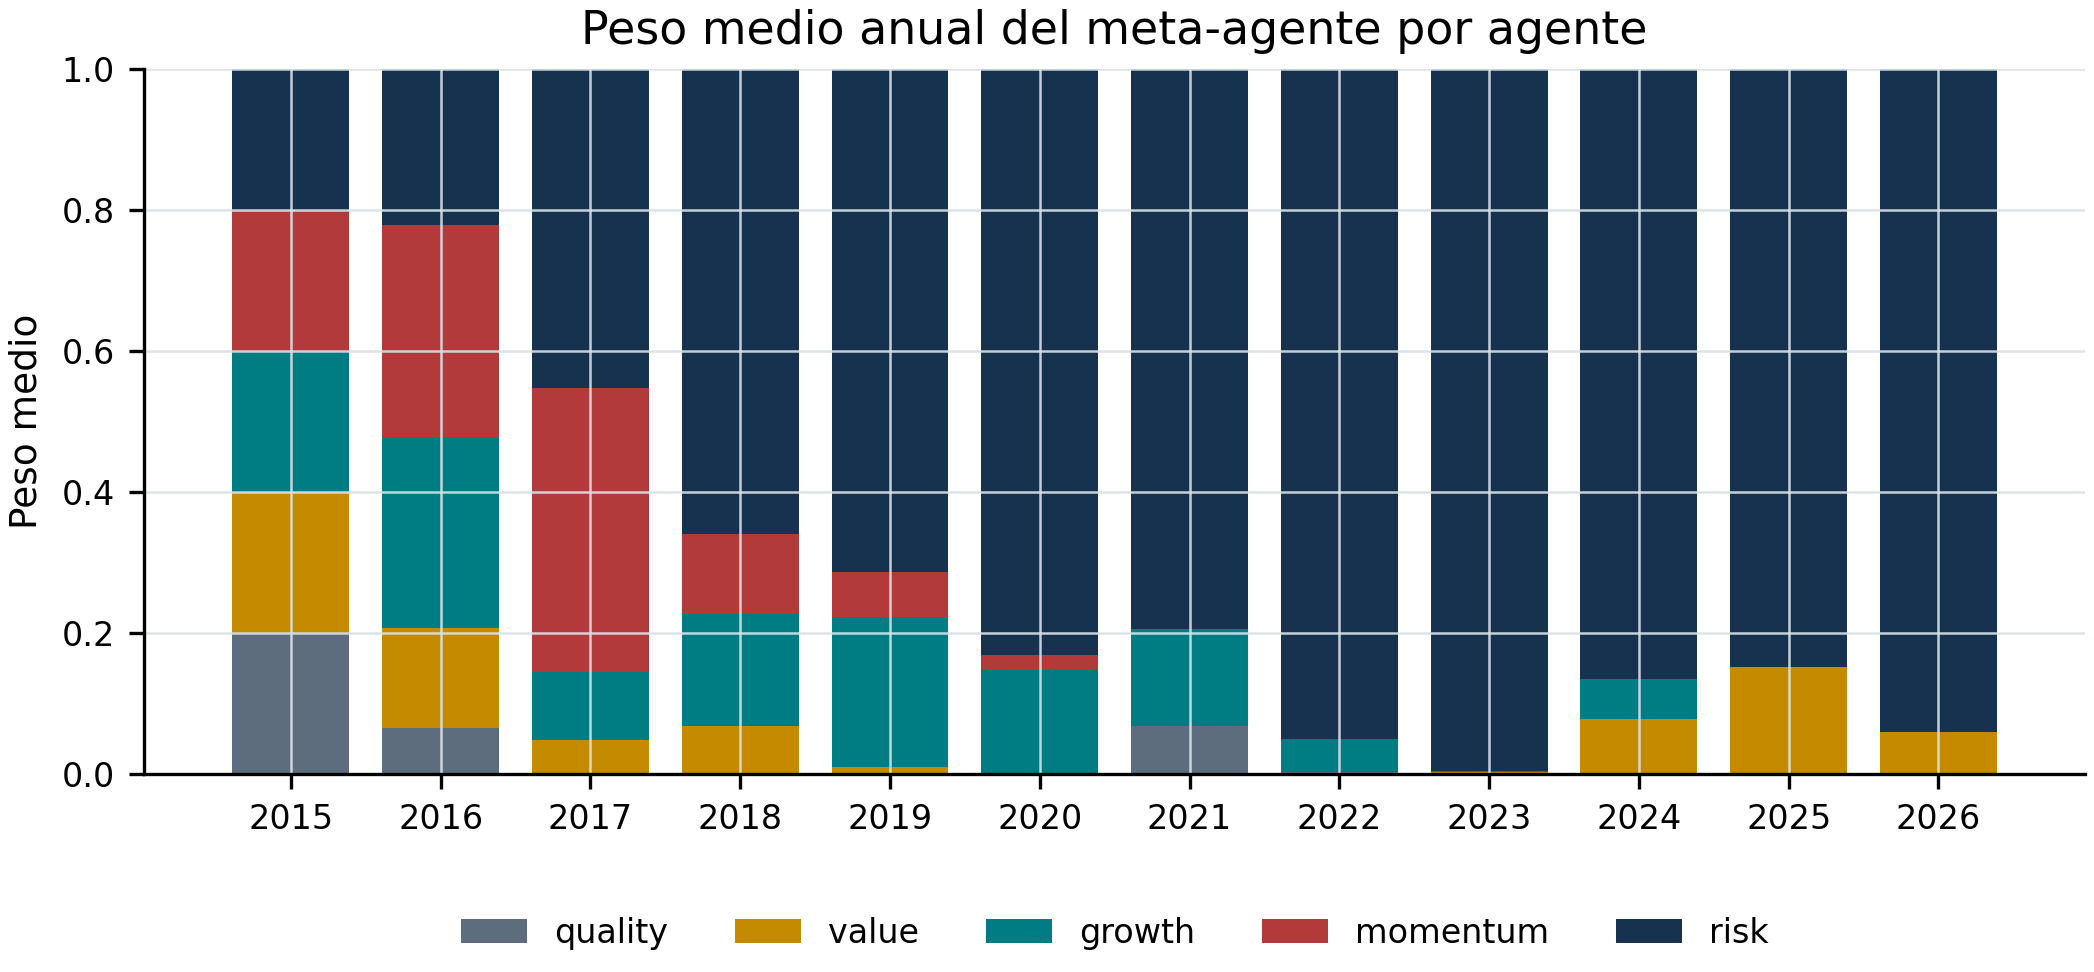
\includegraphics[width=0.94\textwidth]{assets/f05_pesos_anual.png}
  \caption{Peso medio anual asignado por el meta-agente a cada especialista. 2015 corresponde
  íntegramente al reparto uniforme por ausencia de cohortes cerradas. Fuente:
  \artefacto{evidence/meta\_weights.parquet}.}
  \label{fig:pesos-anual}
\end{figure}

La Figura~\ref{fig:pesos-anual} describe un aprendizaje reconocible, y su primer tramo es el más
informativo. En 2015 el reparto es uniforme por construcción. En 2016 el meta concentra en
\textit{momentum}, que acabará siendo el peor especialista de todo el periodo: es un error, y es
exactamente lo que cabe esperar de un sistema que decide con dos años de datos. En 2017 corrige
hacia \textit{risk} (0,45 de media anual), en 2018 lo eleva a 0,66 y a partir de 2020 lo sitúa por
encima de 0,83, alcanzando 0,997 en 2023. Que el sistema se equivoque primero y se corrija después,
sin que nadie intervenga, es la evidencia más directa de que el aprendizaje es real y no una
etiqueta.

\section{Qué mira realmente cada agente}
\label{sec:atribucion-local}

Lo anterior describe el vocabulario que cada agente \emph{recibe}. Qué hace con él es una pregunta
distinta y comprobable: el estudio persiste, para cada acción, fecha, agente y variable, la
contribución local de esa variable a la puntuación resultante
(\artefacto{evidence/agent\_local\_attribution.parquet}, 1.309.618 filas). La
Tabla~\ref{tab:atribucion} resume las tres variables de mayor peso en cada agente.

\begin{table}[H]
  \centering
  \small
  \caption{Variables que más contribuyen a la puntuación de cada agente.}
  \label{tab:atribucion}
  \begin{tabular}{llrrr}
\toprule
Agente & Variable & Contrib. media & Encabeza & Variables distintas \\
\midrule
risk & gap\_21d & 0,0216 & 51,2\% & 12 \\
 & range\_63d & 0,0136 & 26,8\% &  \\
 & max\_drawdown\_252d & 0,0092 & 4,2\% &  \\
value & pb & 0,0155 & 14,2\% & 11 \\
 & pfcf & 0,0105 & 25,6\% &  \\
 & ev\_revenue & 0,0086 & 4,8\% &  \\
growth & cash\_conversion & 0,0147 & 65,8\% & 11 \\
 & roe\_trend & 0,0089 & 4,9\% &  \\
 & sales\_per\_share\_growth\_yoy & 0,0077 & 7,2\% &  \\
quality & asset\_turnover & 0,0147 & 30,2\% & 29 \\
 & receivables\_turnover & 0,0127 & 4,1\% &  \\
 & fcf\_margin & 0,0119 & 27,1\% &  \\
momentum & mom\_volatility & 0,0129 & 22,8\% & 10 \\
 & mom\_acceleration & 0,0127 & 31,6\% &  \\
 & ma\_distance\_to\_high12 & 0,0079 & 12,4\% &  \\
\bottomrule
\end{tabular}

  \caption*{Fuente: \artefacto{evidence/agent\_local\_attribution.parquet}. «Contrib. media» es la
  magnitud media de la contribución local; «Encabeza», la fracción de observaciones en las que esa
  variable fue la primera por importancia. No se reporta el signo medio porque se cancela entre
  acciones y no admite lectura direccional.}
\end{table}

El resultado más relevante afecta a \textit{risk}, que es el agente que domina el sistema y cuyo
predominio el Capítulo~\ref{chap:limitaciones} señala como uno de los puntos menos explicados del
trabajo. La lectura natural sería que reproduce la conocida prima de baja volatilidad. \textbf{Los
datos no la respaldan.}


Las dos variables que mandan son \artefacto{gap\_21d} y \artefacto{range\_63d} --- microestructura
del precio a corto plazo: huecos de apertura y amplitud del rango de negociación ---, que juntas
encabezan el 78\,\% de las observaciones. Las medidas que uno esperaría de una estrategia de baja
volatilidad aparecen después y con menos peso: \artefacto{max\_drawdown\_252d} encabeza el 4,2\,\% y
\artefacto{beta\_252d}, el candidato más obvio, ni siquiera está entre las tres primeras. El agente
no está comprando acciones defensivas en el sentido factorial clásico; está leyendo la estructura
reciente de negociación.

Esta observación es coherente con dos resultados independientes que se presentan más adelante en
este capítulo. Explica por qué la neutralización por catorce controles de estilo
retiene el 86,62\,\% de la señal: si el agente dominante replicase el factor de volatilidad, la
neutralización debería destruir mucho más. Y refuerza la advertencia de no reducir el sistema a una
prima conocida, que hasta ahora se sostenía sólo sobre esa neutralización y ahora tiene además una
explicación mecánica.

\begin{figure}[H]
  \centering
  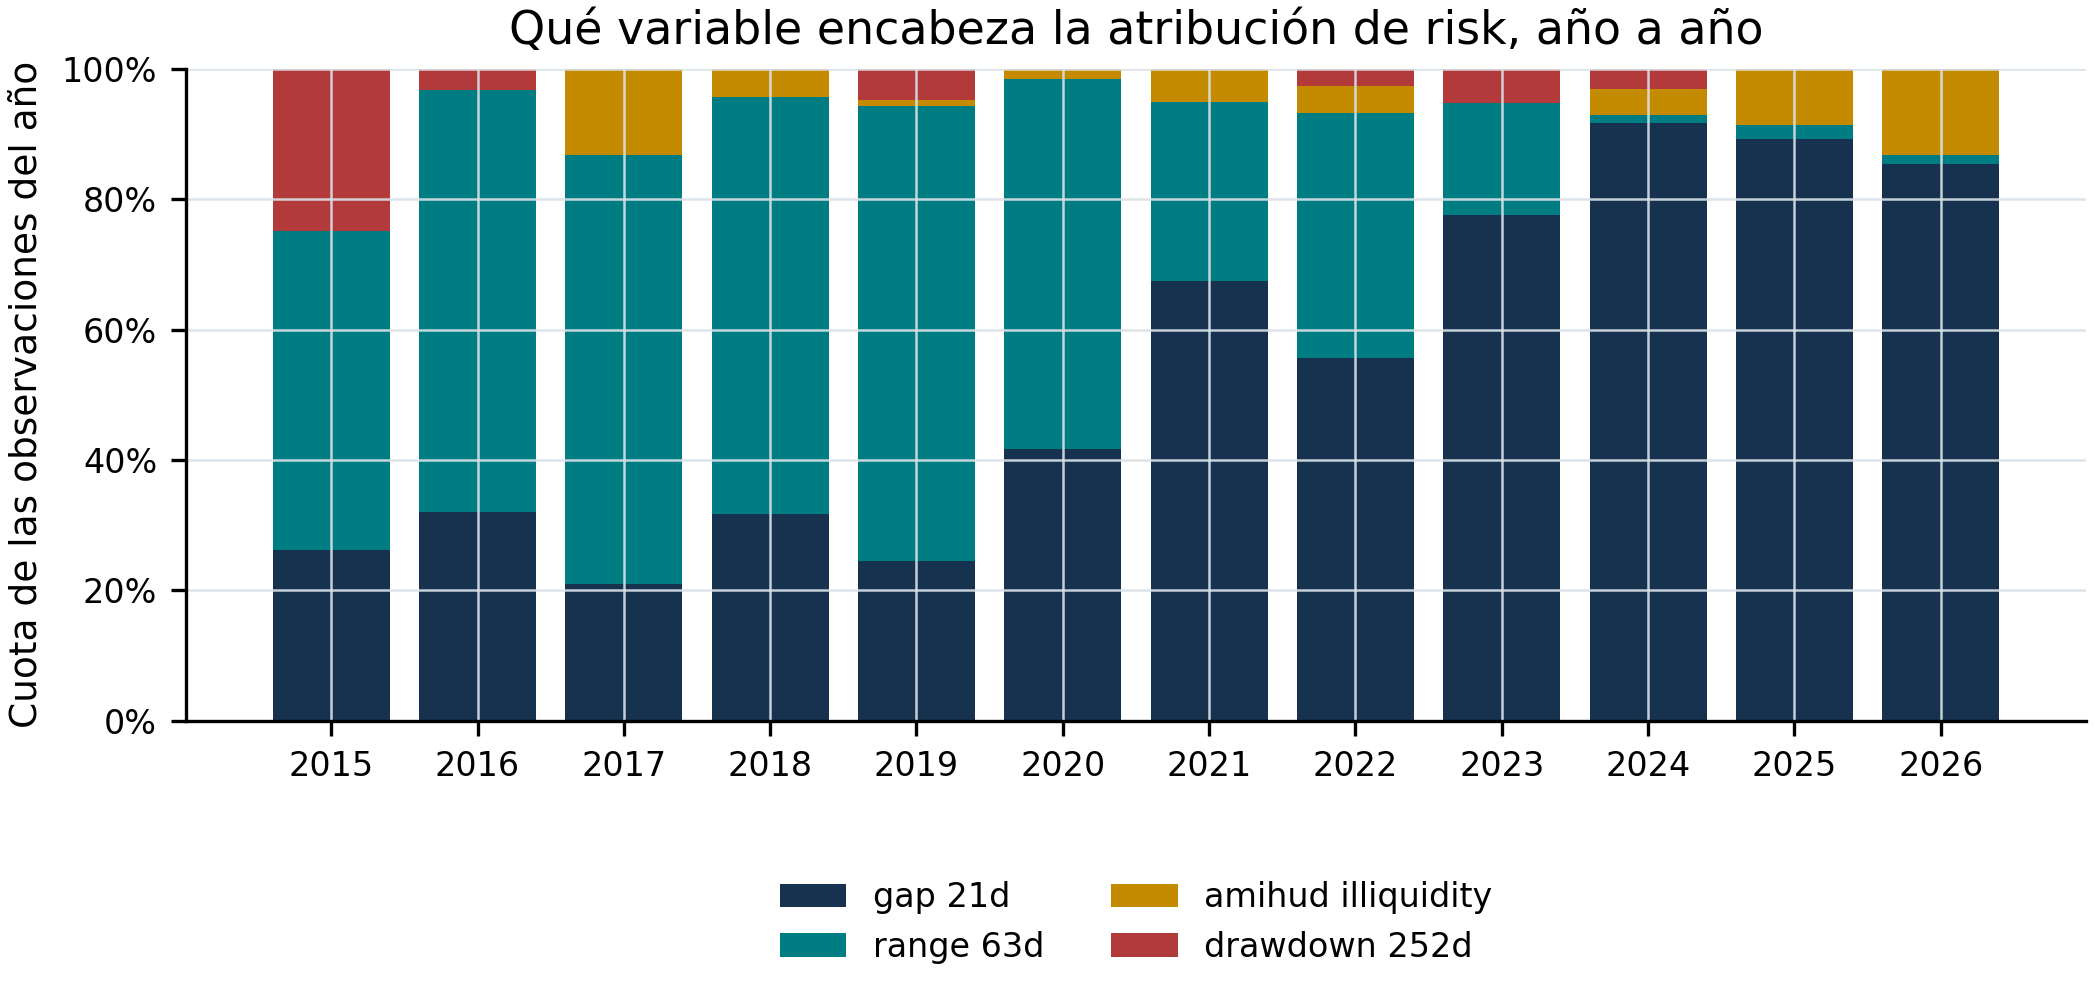
\includegraphics[width=0.92\textwidth]{assets/f05_atribucion_anual.png}
  \caption{Variable que encabeza la atribución de \textit{risk} en cada año, como fracción de las
  observaciones. Fuente: \artefacto{evidence/agent\_local\_attribution.parquet}.}
  \label{fig:atribucion-anual}
\end{figure}

La Figura~\ref{fig:atribucion-anual} añade un matiz importante sobre la concentración del
meta-agente. Aunque \textit{risk} acabe recibiendo más del 95\,\% del peso, no es una apuesta fija:
la variable que lo gobierna cambia con el régimen. \artefacto{range\_63d} domina entre 2017 y 2020
--- el tramo de mayor turbulencia, incluido el desplome de 2020 --- y después se desvanece, mientras
\artefacto{gap\_21d} crece hasta encabezar entre el 64 y el 77\,\% de las observaciones desde 2023. El
sistema reasigna atención dentro del agente aunque el reparto entre agentes esté congelado, lo que
suaviza --- sin eliminarla --- la objeción de que depender de un único especialista equivale a
depender de un único factor.

Conviene declarar el alcance de todo esto. La atribución local es \emph{descriptiva}: dice qué
variables movieron la puntuación, no que esas variables causen el retorno. Ningún contraste de este
capítulo se apoya en ella, y su papel es explicar un resultado ya medido por otros medios, no
sostenerlo.

Una última observación, sobre la amplitud del vocabulario. \textit{Quality} llega a encabezar con
29 variables distintas, casi el triple que \textit{momentum} (10) o \textit{risk} (12), y es a la
vez uno de los peores agentes por Rank-IC (0,0096). No hay aquí evidencia causal --- son cinco
agentes, no una muestra --- pero la asociación es sugerente y apunta en la misma dirección que el
resto del capítulo: repartir la atención entre muchas variables débiles ordena peor que concentrarla
en unas pocas con contenido.
\section{Capacidad predictiva fuera de muestra}

En la ventana de selección 2015--2024, el sistema alcanza Rank-IC medio 0,1090, IC-IR 0,851 y
74,36\% de cohortes positivas. Son 117 cohortes mensuales, aunque el horizonte de doce meses deja
aproximadamente nueve observaciones independientes efectivas: ambos números deben leerse juntos.
El estadístico Newey--West es 3,46. La evidencia mide la calidad de la ordenación transversal, no la
rentabilidad de una única cartera.

Estas cifras corresponden a la tercera y última pasada de la cadena de estudios descrita en la
Sección~\ref{sec:cadena-studies}. Las tres pasadas mejoraron de forma monótona dentro de esta
ventana --- 0,1000, 0,1074 y 0,1090 de Rank-IC ---, y esa mejora sostenida es precisamente lo que
obliga a mirar con atención la era reservada más adelante en este capítulo.

\begin{figure}[H]
  \centering
  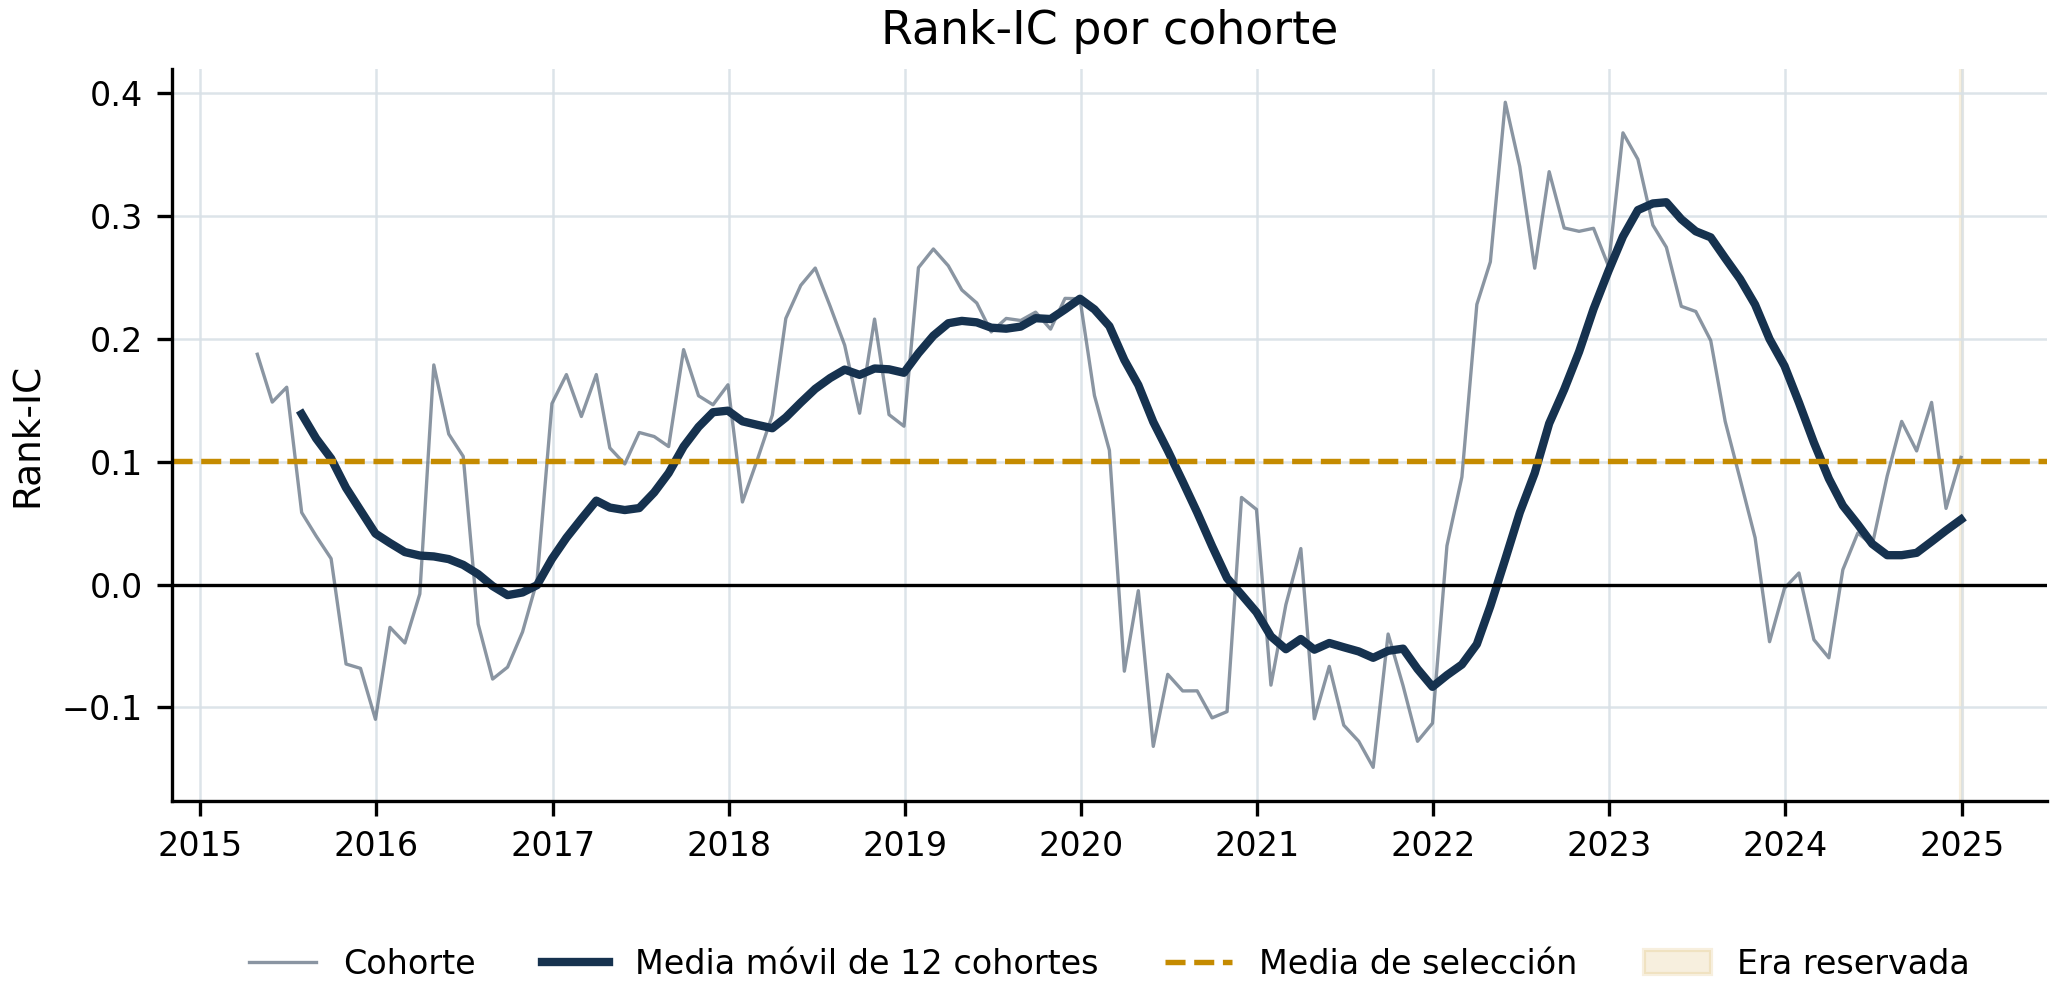
\includegraphics[width=0.96\textwidth]{assets/f07_rankic_serie.png}
  \caption{Rank-IC por cohorte. La banda dorada identifica la era reservada, que no intervino en
  ninguna decisión. Fuente: \texttt{evidence/summary.json}.}
  \label{fig:rankic-serie}
\end{figure}

La comparación limpia se hace contra scores deterministas calculados sobre el mismo panel y con las
mismas restricciones temporales. El mejor, \texttt{garp\_score}, obtiene 0,0130; el sistema lo
multiplica aproximadamente por ocho. No se infiere de ello que los factores clásicos sean inútiles,
sino que, bajo este universo y este protocolo, una combinación no lineal y temporalmente cerrada
ordena mejor los retornos futuros que las fórmulas fijas.

\begin{table}[H]
  \centering
  \caption{Sistema frente a baselines deterministas.}
  \label{tab:baselines}
  \begin{tabular}{lrr}
\toprule
Señal & Rank-IC & Cohortes positivas \\
\midrule
Sistema (meta final) & 0,1067 & 76,07\% \\
garp\_score & 0,0119 & 62,21\% \\
growth\_score & 0,0022 & 51,91\% \\
momentum\_score & -0,0002 & 52,67\% \\
quality\_score & 0,0024 & 52,29\% \\
value\_score & 0,0026 & 48,85\% \\
\bottomrule
\end{tabular}

  \caption*{Fuente: \texttt{attribution.json} y \texttt{evidence/summary.json}.}
\end{table}

Por eras, el Rank-IC es 0,0999 en 2015--2018, 0,0506 en 2019--2021 y 0,1788 en 2022--2024. La
señal se debilita a la mitad en el régimen intermedio, pero no cambia de signo ni depende de la era
final. Esta heterogeneidad justifica reportar series y no una única media agregada, y advierte de
antemano que una media de diez años puede ocultar regímenes en los que el sistema ordena bastante
peor de lo que su cifra agregada sugiere.

\subsection*{La cola superior frente a la ordenación completa}

El Rank-IC resume la calidad de toda la ordenación transversal, pero la cartera sólo compra el
extremo superior. Conviene por tanto comprobar si la ventaja se concentra donde efectivamente se
utiliza. La Tabla~\ref{tab:cola} descompone el comportamiento de la cola por era.

\begin{table}[H]
  \centering
  \small
  \caption{Comportamiento de la cola superior de la ordenación, por era.}
  \label{tab:cola}
  \begin{tabular}{lrrrrrr}
\toprule
Era & Rank-IC & Top 10 & Decil sup. & Universo & Sup. menos inf. & Cohortes \\
\midrule
2015-2018 & 0,0999 & 5,78\% & 4,02\% & -0,26\% & 5,24\% & 45 \\
2019-2021 & 0,0506 & 0,56\% & 1,22\% & -0,00\% & 5,31\% & 36 \\
2022-2024 & 0,1788 & -0,13\% & -1,34\% & -6,47\% & 13,97\% & 36 \\
2025-2026 & 0,0441 & -7,61\% & -7,67\% & -1,85\% & 11,33\% & 6 \\
\bottomrule
\end{tabular}

  \caption*{Fuente: \artefacto{evidence/rank\_tail\_diagnostics.parquet}. «Top 10» es el exceso medio
  de las diez primeras posiciones; «Universo» el de todo el panel. Diagnóstico, no criterio de
  selección.}
\end{table}

La lectura relevante es que el decil superior bate al universo en las tres eras de selección, de
modo que la ventaja no procede exclusivamente de acertar la cola inferior --- que una cartera
\textit{long-only} no puede explotar. La Figura~\ref{fig:cola} muestra esa diferencia cohorte a
cohorte: es ruidosa, como corresponde a un estadístico calculado sobre unas pocas decenas de
valores, pero su media móvil se mantiene por encima de cero durante casi toda la ventana.

\begin{figure}[H]
  \centering
  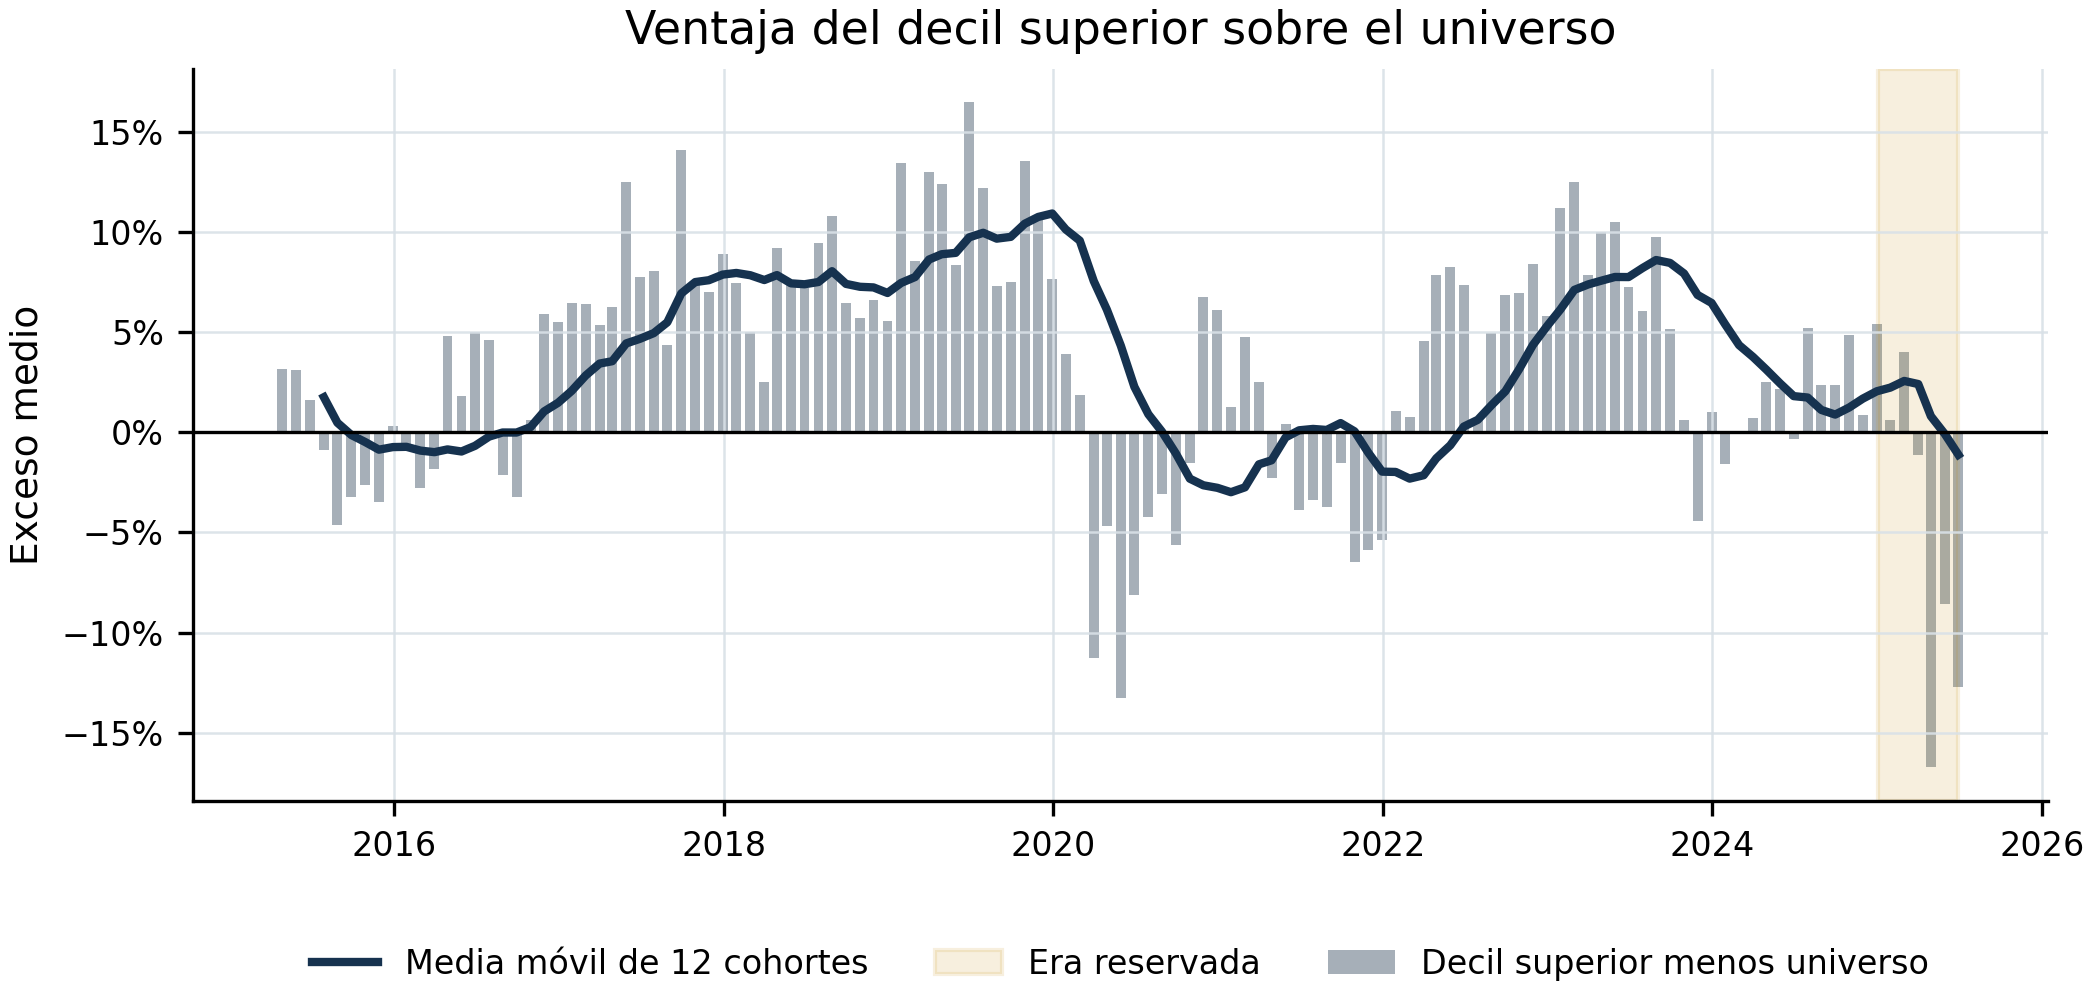
\includegraphics[width=0.94\textwidth]{assets/f07_cola.png}
  \caption{Exceso del decil superior sobre el universo, por cohorte. Fuente:
  \artefacto{evidence/rank\_tail\_diagnostics.parquet}.}
  \label{fig:cola}
\end{figure}

Existe además un diagnóstico que el sistema calcula en cada snapshot para su propio uso: el Rank-IC
contraído sobre las cohortes ya cerradas en ese momento. Es la única medida de calidad de señal
disponible \textit{en tiempo real}, puesto que no utiliza información posterior a la fecha. La
Figura~\ref{fig:salud} la representa con dos memorias distintas.

\begin{figure}[H]
  \centering
  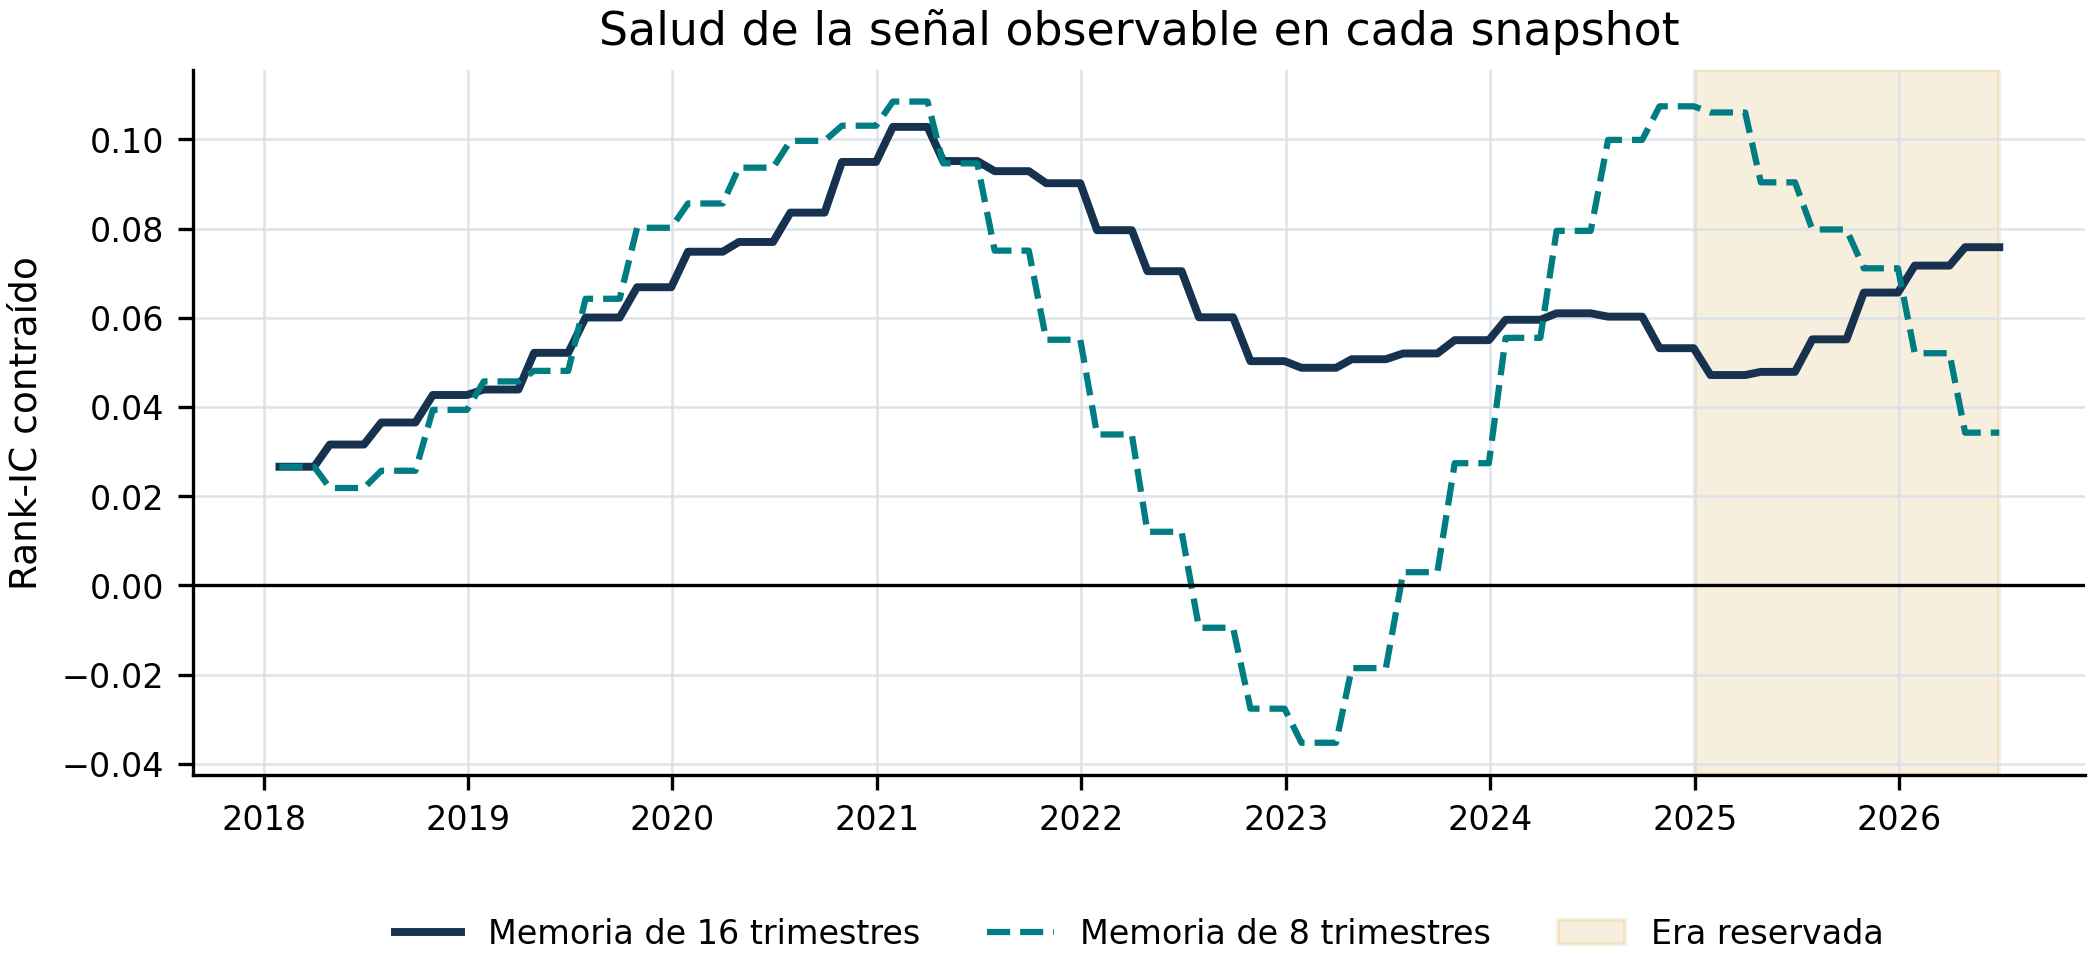
\includegraphics[width=0.94\textwidth]{assets/f07_salud.png}
  \caption{Salud de la señal observable en cada snapshot, con memoria de dieciséis y de ocho
  trimestres. Fuente: \artefacto{evidence/signal\_health.parquet}.}
  \label{fig:salud}
\end{figure}

La comparación entre ambas memorias es informativa por sí misma. La ventana corta reacciona antes a
los cambios de régimen, pero también oscila más y llega a cruzar cero en episodios que la ventana
larga apenas registra. Esta diferencia explica por qué el catálogo trata la longitud de la memoria
del meta-agente como una variable a decidir con evidencia y no como una constante razonable: ambas
opciones tienen un coste, y la elección entre reaccionar antes o estimar con menos varianza no
puede resolverse por intuición.
\section{Atribución, factores y resultado no superado}

Dos contrastes independientes preguntan lo mismo desde ángulos distintos: ¿es la señal una réplica
de estilos ya conocidos?

El primero neutraliza. Regresando la señal contra catorce controles de valoración, rentabilidad,
crecimiento, volatilidad y beta --- listados en el Anexo~\ref{anexo:evidencia} --- y recalculando
después el Rank-IC, éste baja de 0,1177 a 0,1019. La pérdida del 13,38\,\% indica que parte de la
señal comparte información con esos controles, como sería esperable en un sistema que usa ratios
económicos; la retención del \textbf{86,62\,\%} muestra que no se agota en ellos.

El segundo regresa los retornos contra cinco factores de estilo con errores Newey--West de doce
retardos. Sobre las 117 cohortes de selección el $R^2$ es 0,017 y ninguna carga alcanza
significación --- la mayor en valor absoluto es momentum, con $-0{,}105$ ---, de modo que no hay
exposición factorial estable. Su alfa por periodo, 0,27\,\% con $t=1{,}44$, tampoco es significativo
de forma aislada. Los factores de tamaño e inversión no son construibles con las fuentes disponibles
y se declaran no replicables en lugar de sustituirse por un sucedáneo no auditable.

Las dos mitades deben leerse juntas, porque acotan la afirmación por ambos lados: no hay evidencia
suficiente para atribuir la señal a un factor clásico, ni tampoco para afirmar que genere alfa por
sí misma. La conclusión prudente es que la evidencia es compatible con una señal parcialmente
distinta de los factores implementados, no que se haya descubierto una prima nueva y causal.

Conviene precisar el alcance del segundo contraste, porque su procedencia difiere del resto del
capítulo: se calcula sobre la serie de retornos de la cartera de referencia del Model Study, que no
es la que el trabajo adopta. Eso lo hace válido para la pregunta que aquí se formula --- si la señal
se explica por estilos conocidos, algo que no depende de cuántas posiciones se compren --- pero no
para describir la cartera final, cuyas cifras se presentan íntegramente en el
Capítulo~\ref{chap:resultados-economicos} desde su propia evidencia.

El Deflated Sharpe de 0,682, inferior a 0,95, es la limitación empírica más importante, y su valor
ha empeorado respecto de las pasadas anteriores de la cadena precisamente porque la cadena existe:
el estadístico penaliza el Sharpe por el número de configuraciones ensayadas, y encadenar estudios
multiplica ese número. Recuerda, por tanto, que una rentabilidad histórica seleccionada entre
decenas de alternativas merece escepticismo adicional. No contradice el test de permutación del
Rank-IC: ambos examinan objetos diferentes. El primero limita una afirmación de rentabilidad
ajustada por riesgo; el segundo apoya que el ranking no se comporta como ruido puro. Que uno se
debilite mientras el otro se mantiene es exactamente el patrón esperable cuando se busca más: la
evidencia de \emph{señal} resiste y la de \emph{rentabilidad} se encarece.
\section{Robustez: aprendizaje y no suerte}

La Tabla~\ref{tab:robustez} resume ocho contrastes predefinidos. Siete respaldan la capacidad
predictiva; el Deflated Sharpe no alcanza su umbral de 0,95. Reportar este último resultado evita
convertir la robustez en una lista selectiva de éxitos: la evidencia de señal y la evidencia de
rentabilidad ajustada por multiplicidad no tienen la misma fuerza.

\begin{table}[H]
  \centering
  \caption{Resumen de contrastes de robustez.}
  \label{tab:robustez}
  \begin{tabular}{llc}
\toprule
Contraste & Resultado & Veredicto \\
\midrule
Permutación & $p=0,0001$; 9.999 réplicas & Supera \\
Placebos & Rank-IC entre $-0,0081$ y $0,0013$ & Supera \\
Bootstrap & IC 95\% $[0,0425; 0,1723]$ & Supera \\
Exclusión de eras & Rank-IC entre $0,0780$ y $0,1350$ & Supera \\
Semillas & Rango de Rank-IC $0,0015$ & Supera \\
Aleatorias con riesgo & Percentil $96,8$ & Supera \\
Neutralización & Retiene 86,62\% de la señal & Supera \\
Deflated Sharpe & $0,682 < 0,95$ & No supera \\
\bottomrule
\end{tabular}

  \caption*{Fuente: \texttt{robustness.json} y \texttt{attribution.json}. Los contrastes de señal no
  dependen de la cartera; el Deflated Sharpe y las carteras aleatorias, que sí, están calculados
  sobre la cartera del Model Study.}
\end{table}


El test de permutación entrega $p=0,0001$ con 9.999 réplicas y corrección +1: ninguna réplica
igualó el Rank-IC observado. La permutación destruye únicamente el vínculo entre el orden predicho
y el retorno futuro dentro de cada cohorte, conservando el calendario, el número de empresas y la
distribución transversal de los retornos. Responde por tanto a una pregunta muy concreta: ¿puede
surgir un Rank-IC como el observado sin ninguna asociación predictiva? Con 9.999 réplicas y ninguna
que lo alcance, la respuesta empírica es que no.

Los cinco placebos de etiqueta son complementarios y atacan otra objeción. Conservan la maquinaria
completa de features, agentes, meta-agente y cartera, pero sustituyen la etiqueta por una barajada.
Si alguna parte del \textit{pipeline} fabricase señal por sí misma --- una normalización mal
cerrada, una fuga temporal, un artefacto de la validación ---, los placebos deberían mostrar una
magnitud comparable a la observada. Quedan entre $-0{,}0081$ y $+0{,}0013$, es decir, indistinguibles
de cero y un orden de magnitud por debajo del sistema.

\begin{figure}[H]
  \centering
  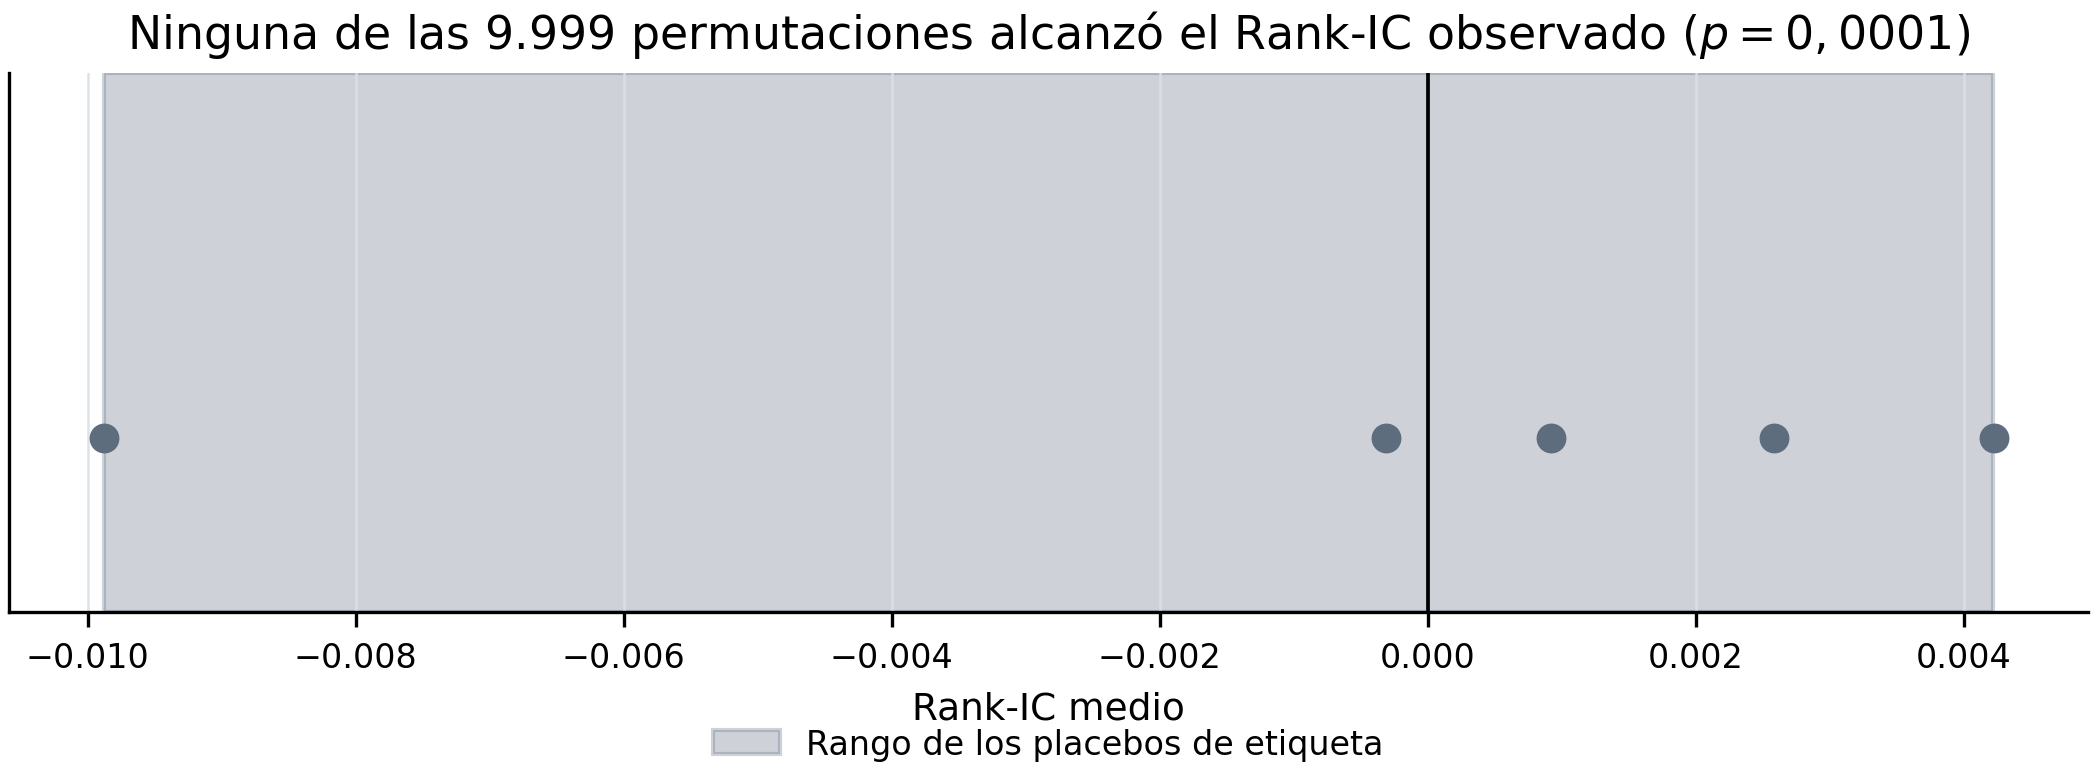
\includegraphics[width=0.94\textwidth]{assets/f07_permutacion.png}
  \caption{Situación del Rank-IC observado frente al rango de los placebos de etiqueta y al
  resultado del contraste de permutación. Fuente: \artefacto{robustness.json}.}
  \label{fig:permutacion}
\end{figure}

La Figura~\ref{fig:permutacion} representa la distribución nula completa: el estudio persiste los
estadísticos de las 9.999 permutaciones, no sólo el $p$-valor resultante, de modo que puede verse
dónde cae el Rank-IC observado dentro de la nube de permutaciones y no únicamente que la supera. El
$p$-valor del texto se recalcula exactamente desde esas réplicas. El Anexo~\ref{anexo:evidencia}
detalla qué se guarda de cada contraste.

El \textit{bootstrap} por bloques y la exclusión de eras responden a una tercera objeción: que una
media positiva esté dominada por meses correlacionados o por un subperiodo excepcional. Manteniendo
bloques de doce cohortes --- la longitud del horizonte, precisamente para no romper la dependencia
que el solapamiento induce ---, el intervalo al 95\,\% es $[0,0425;\,0,1723]$ y excluye cero.
Eliminando por completo cualquiera de las tres eras, la media permanece entre 0,0780 y 0,1350. La
Figura~\ref{fig:bootstrap} reúne ambos contrastes.

\begin{figure}[H]
  \centering
  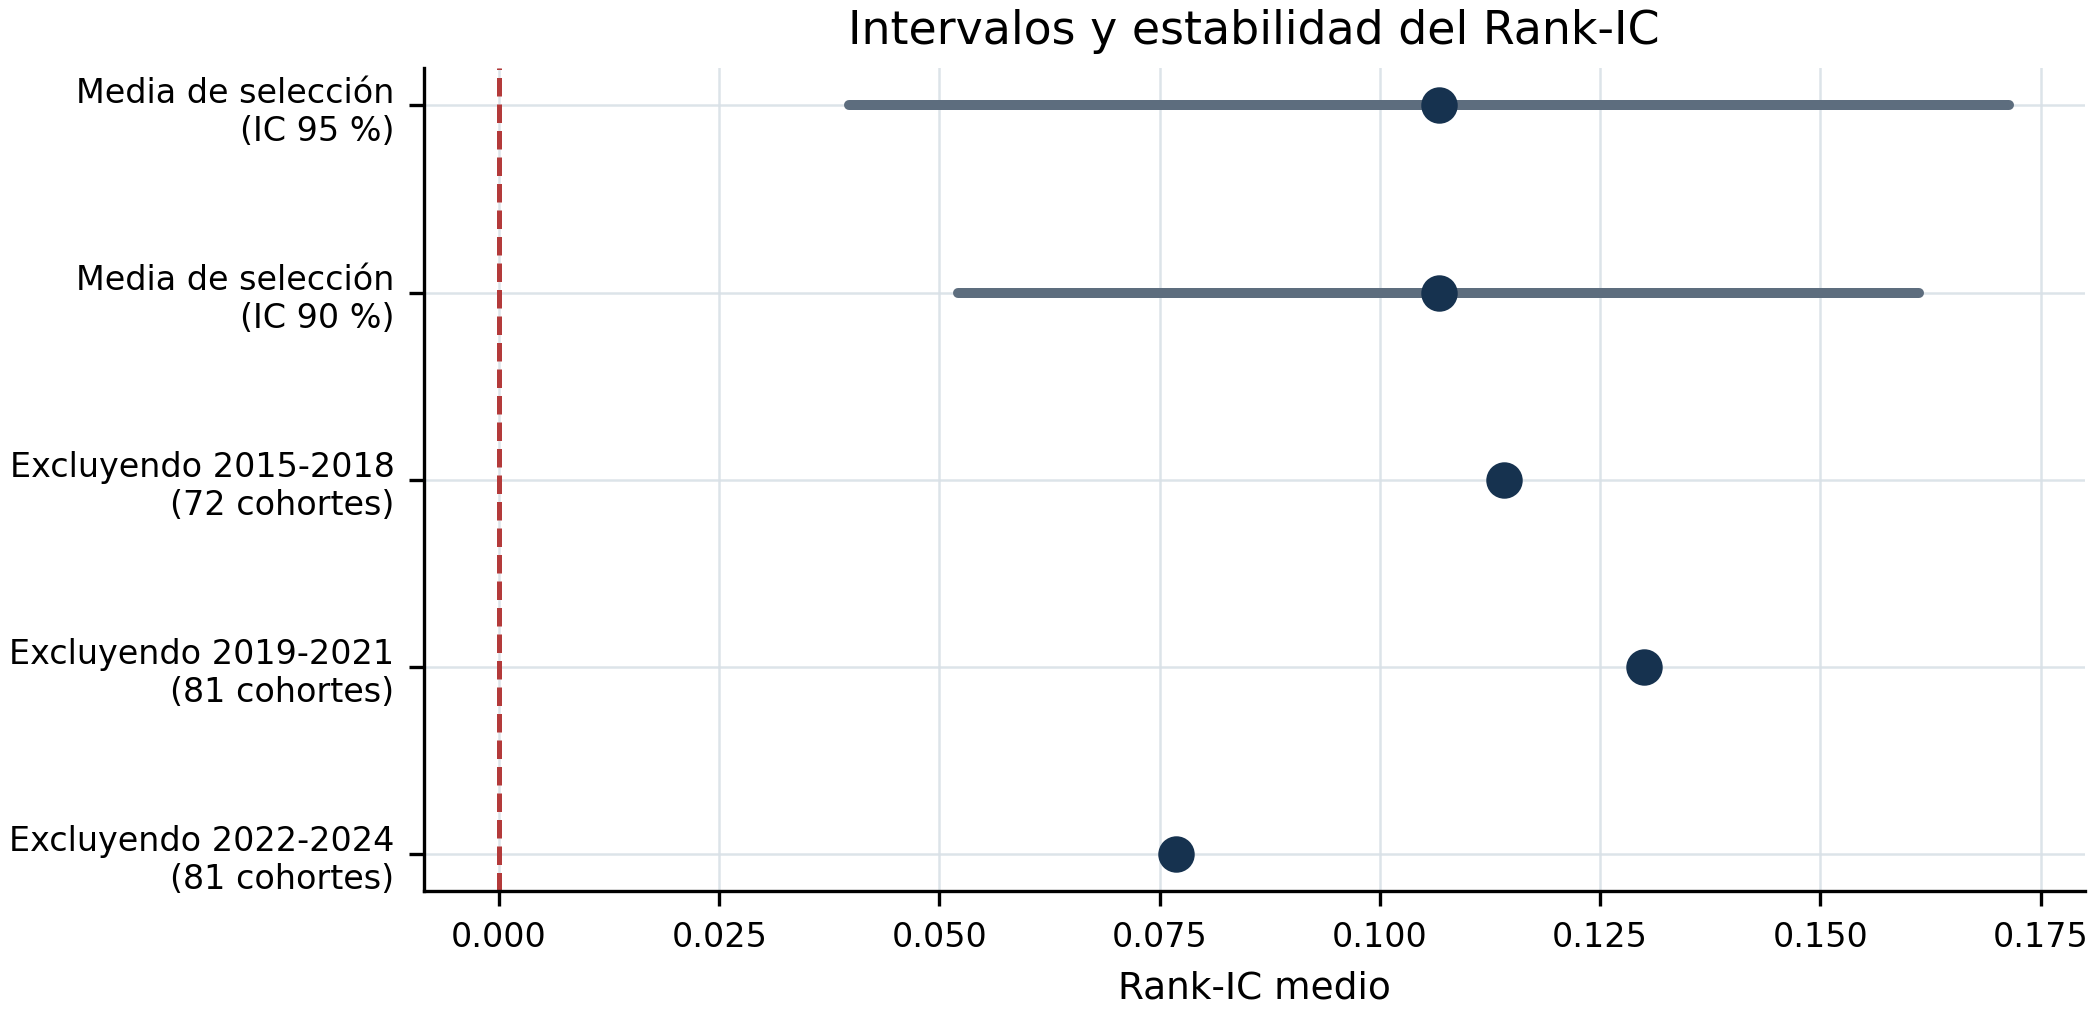
\includegraphics[width=0.94\textwidth]{assets/f07_bootstrap.png}
  \caption{Intervalos de confianza del Rank-IC y estabilidad ante la exclusión de eras completas.
  Fuente: \artefacto{robustness.json}.}
  \label{fig:bootstrap}
\end{figure}

El contraste más exigente de la era 2022--2024 merece una nota: al excluirla, el Rank-IC cae a
0,0780, el valor más bajo de los tres. Es coherente con que sea la era de mayor señal (0,1788) y no
indica fragilidad, sino que esa era aporta una parte apreciable de la evidencia. La conclusión
prudente es que el resultado no depende de ninguna era, pero tampoco es homogéneo entre ellas.

La estabilidad entre semillas ataca una posibilidad distinta: que el resultado dependa de una
inicialización afortunada del \textit{boosting}. En las tres semillas ensayadas el rango de Rank-IC
es 0,0015 y no cruza cero. La Figura~\ref{fig:semillas} muestra, sin embargo, que la conclusión
económica es bastante más frágil que la predictiva: el exceso geométrico varía apreciablemente más
que el Rank-IC en términos relativos. Esta asimetría es la misma que motivó introducir el conjunto
de semillas durante el desarrollo, según se documenta en el Anexo~\ref{anexo:desarrollo}.

\begin{figure}[H]
  \centering
  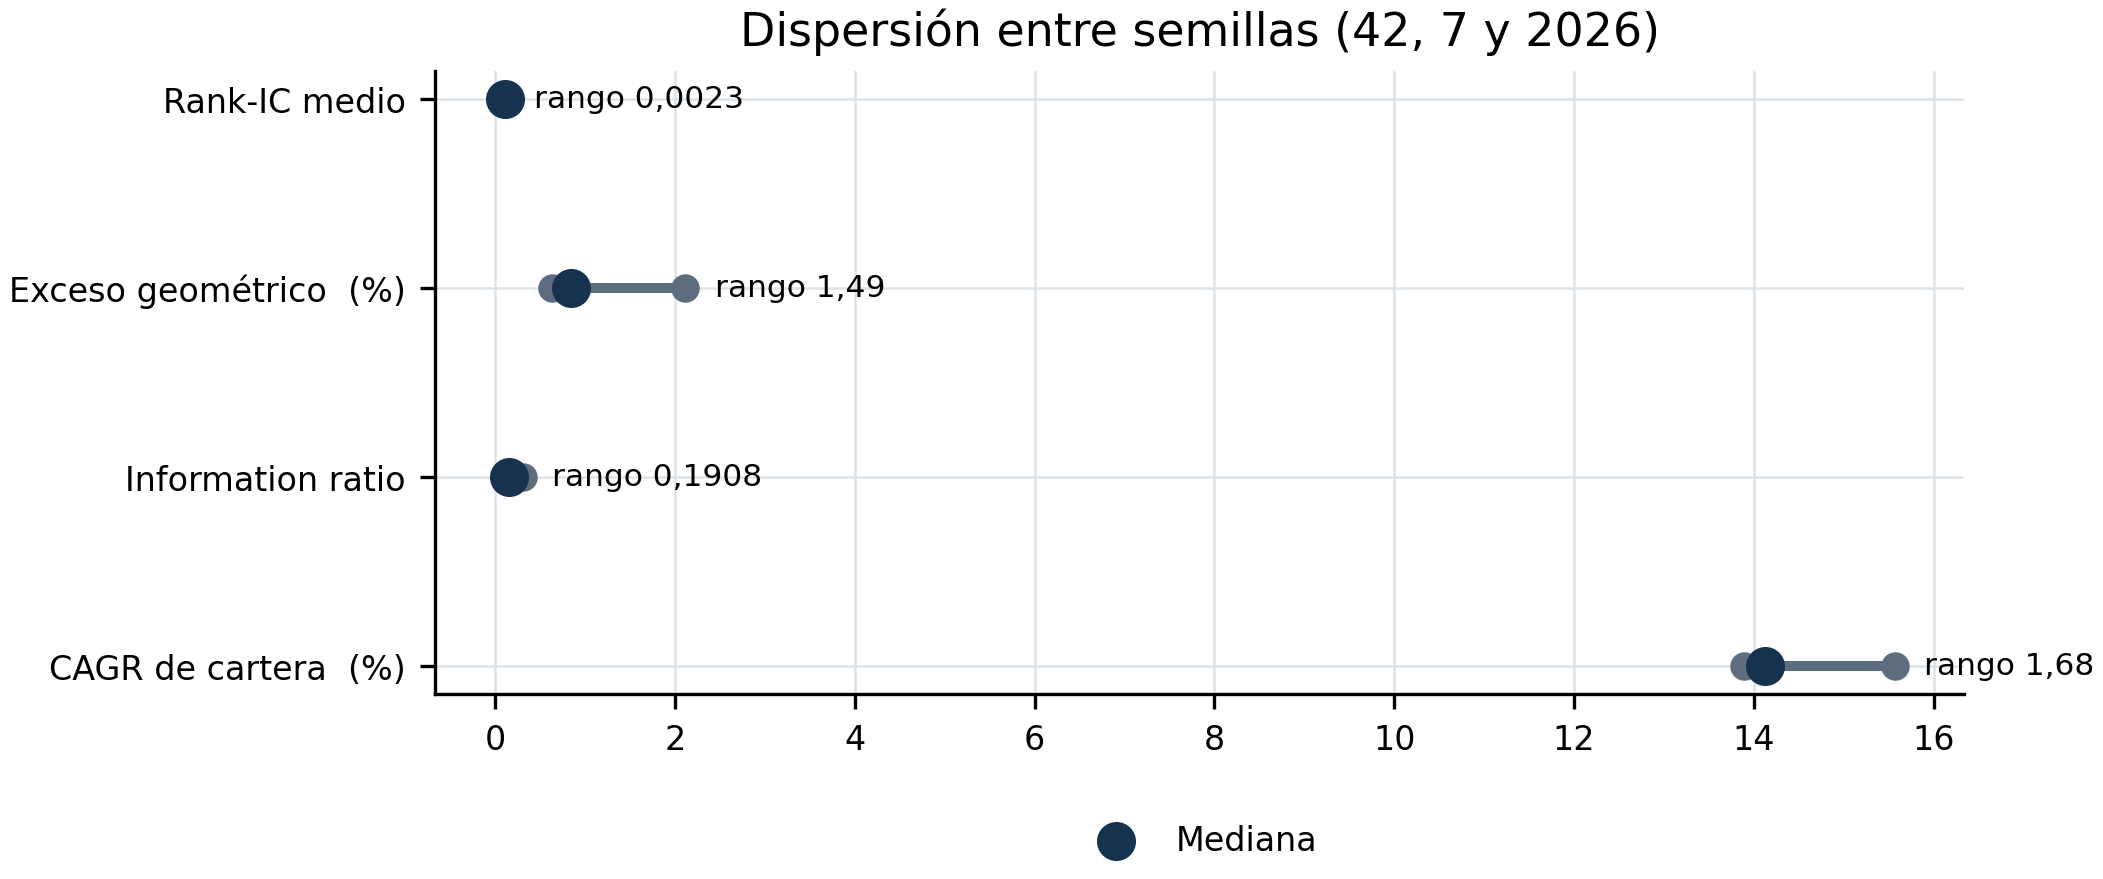
\includegraphics[width=0.92\textwidth]{assets/f07_semillas.png}
  \caption{Dispersión de las métricas principales entre las tres semillas ensayadas. Fuente:
  \artefacto{robustness.json}.}
  \label{fig:semillas}
\end{figure}

Frente a 1.000 carteras aleatorias de riesgo emparejado, la cartera del modelo ocupa el percentil
96,8, con un CAGR del 15,56\,\% frente a una mediana aleatoria del 9,23\,\%. El contraste aleatorio
general no se usa como prueba favorable, y conviene explicar por qué: su percentil 95 de CAGR es
75,06\,\%, dominado por carteras que por azar concentraron alguna superviviente extraordinaria. Un
nulo con esa cola no es un \textit{benchmark} informativo, y presentarlo como si el modelo «sólo»
alcanzase el percentil 76,1 sería tan engañoso como omitirlo. La
Figura~\ref{fig:aleatorias} muestra los dos escenarios juntos precisamente para que la diferencia
sea visible.

\begin{figure}[H]
  \centering
  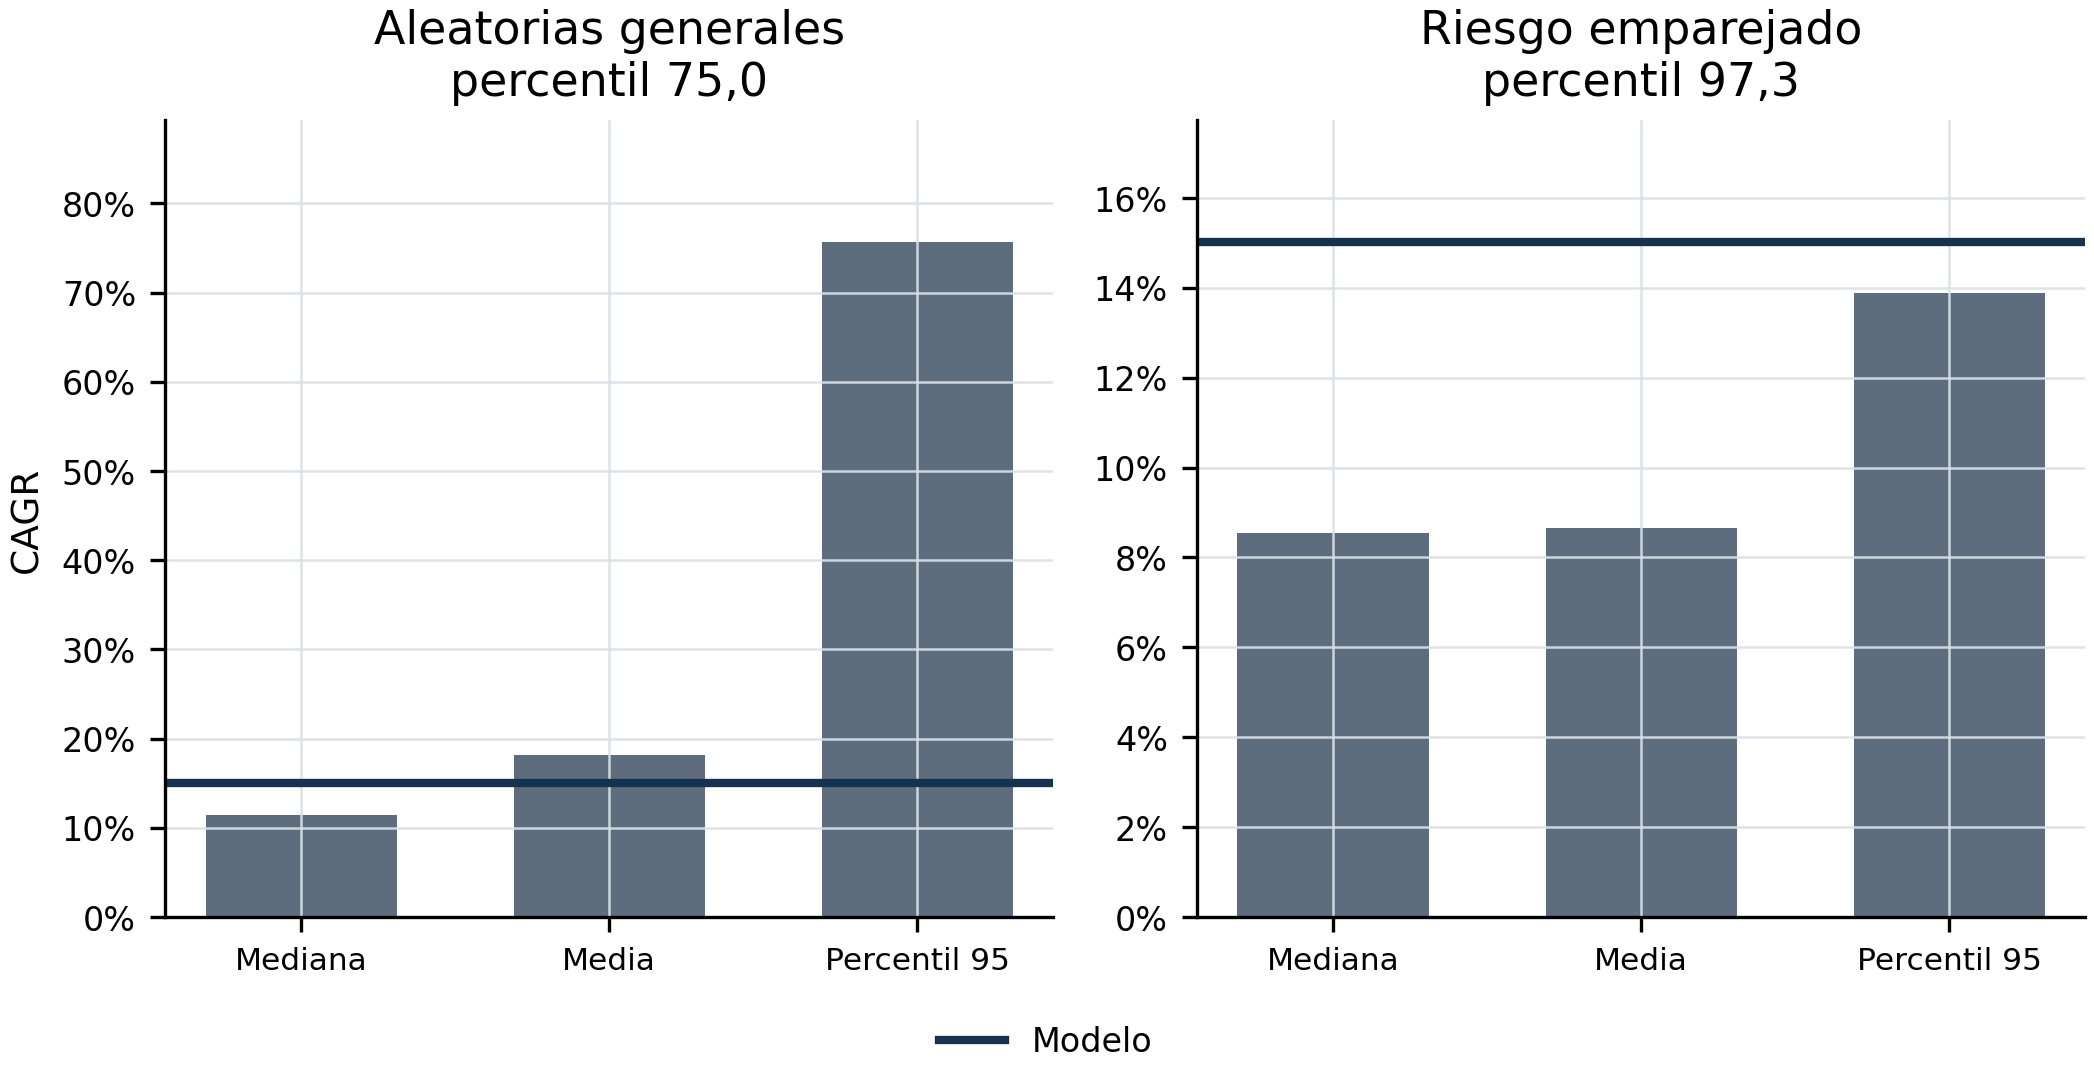
\includegraphics[width=0.92\textwidth]{assets/f07_aleatorias.png}
  \caption{Cartera del modelo frente a 1.000 carteras aleatorias, en el escenario general y con
  riesgo emparejado. Fuente: \artefacto{robustness.json}.}
  \label{fig:aleatorias}
\end{figure}

\section*{Qué queda establecido y qué no}

Conviene recapitular el balance del capítulo, porque su conclusión es afirmativa pero con un
perímetro estrecho que el resto del documento respeta.

Queda establecido que la ordenación existe. El Rank-IC de 0,1090 con $t$ de Newey--West 3,46 no es
un artefacto de la agregación: ninguna de 9.999 permutaciones lo alcanza, los cinco placebos de
etiqueta quedan un orden de magnitud por debajo, el intervalo bootstrap por bloques excluye cero,
la conclusión sobrevive a eliminar cualquier era completa y las tres semillas coinciden dentro de
0,0015. Queda establecido también que no se agota en controles conocidos: la neutralización por
catorce variables de estilo retiene el 86,62\,\% de la señal, y la atribución local explica por qué
--- el agente dominante lee microestructura de precio a corto plazo, no la prima de baja volatilidad
que su nombre sugiere.

No queda establecido que la arquitectura multi-agente esté justificada por estos datos: el agente
\textit{risk} aislado ordena mejor que el meta que lo contiene, y el meta acaba asignándole más del
95\,\% del peso. Tampoco queda establecida ninguna afirmación de rentabilidad ajustada por
multiplicidad: el Deflated Sharpe de 0,682 no alcanza su umbral, y encadenar tres estudios ha
encarecido esa exigencia en lugar de aliviarla. Y no queda establecido que la señal se mantenga
fuera de la ventana de decisión con la fuerza que muestra dentro: en la era reservada el Rank-IC
sigue siendo positivo, $+0{,}0441$, pero descansa sobre seis cohortes.

Con esto queda contestada la primera pregunta del trabajo. La segunda es independiente y no se
deduce de la anterior: si una cartera real puede expresar esa ordenación sin destruirla por el
camino. Nada de lo visto hasta aquí la anticipa --- el Rank-IC no depende de cuántas posiciones se
compren ni de cuánto cueste rotarlas ---, y la respuesta resultará depender de esa construcción
mucho más de lo que cabría esperar. A ella responde el Capítulo~\ref{chap:resultados-economicos}.
